%!TEX root = ThesisLKN.tex
\chapter{Summary of Results}

This thesis focuses on human tracking in indoor environments, such as offices and factories. In those environments, since there exists static obstacles, e.g., walls, tables, the tracking algorithm needs to differentiate between static obstacles and moving humans. One general tracking algorithm from literature is called as \textit{Bayesian Occupancy Filter}(BOF). It represents the environment as a grid map, and it predicts the occupancy probability of each cell for every time step. An improved version of BOF is \textit{Bayesian Occupancy Filter Using Map knowledge}(BOFUM). As its name indicates, it utilizes prior map knowledge about how likely a tracking object might be on different locations on a given map. 

\begin{figure}[ht]
  \centering
    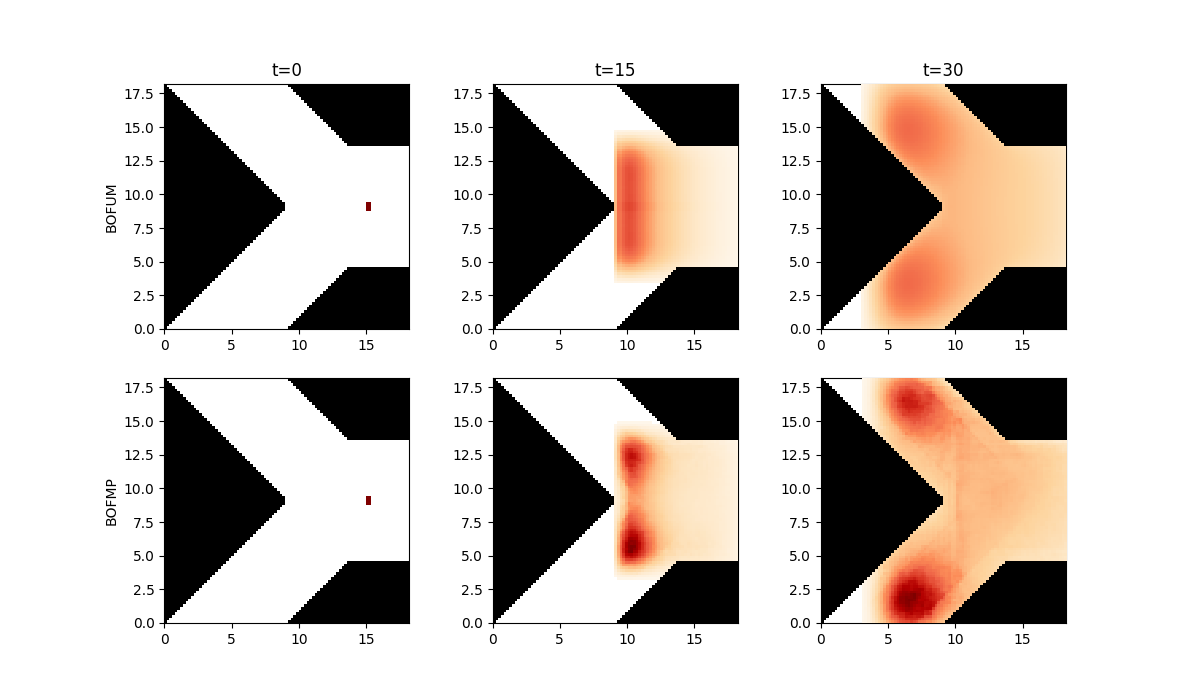
\includegraphics[width=\textwidth]{figures/idea.png}
    \caption{Occupancy predictions for BOFUM and our proposed BOFMP after several time steps. The map shows a T-section. At $t=0$, a person is shown as a red rectangle and with initial velocity towards left. At $t=15$, the person encounters intersection. BOFUM has no information about human motion pattern, and continues to propagate occupancy towards left. Our BOFMP knows that humans are likely to turn to either upper or lower corridors. At $t=30$, since occupancies going left vanish due to the wall, BOFUM predicts occupancies in corridors, but they are biased towards walls on the left. Our BOFMP predicts more occupancies in the middle of corridors, since it knows humans are more likely to walk in the middle.}
    \label{fig:idea}
\end{figure}

Human trajectories in indoor environment follow some motion patterns. For example, when there is corridor, humans tend to walk in the middle of the corridor, instead of walking besides the walls. To incoporate this human motion into tracking algorithm, we proposed \textit{Bayesian Occupancy Filte Using Motion Pattern}(BOFMP). The idea is shown in Figure \ref{fig:idea}.

The main contributions of this thesis work are summarized as following:

\begin{my_enumerate}
\item Neural Network Training.
\item Human Trajectory Simulation.
\item Object Tracking using Bayesian Occupancy Filter
\item Comparision between BOFUM and BOFMP
\end{my_enumerate}

\section{ Neural Network Training}  To capture  human motion patterns, we trained neural networks to learn how a walking person changes directions at different locations on a given map. Mathmatically, there are two ways to represent the motion pattern, either using conditional probability or joint probability. For the former one, given a grid map as input, the network learns for each given grid cell \( c \) on the map, the probabilities of next possible velocity \( V \) conditioned on last velocity \( V^- \):

\[ P_c\{V | V^-\} \] 

Alternatively, the network can also learn the joint probability:

\[ P_c\{V , V^-\} \]

Theoretically, it is always better to have joint probability, since conditional probability can be caculated from joint probability by marginalization and Baye's rule. However, due to reasons explained in Section \ref{section:hms}, we are not able to get accurate joint probabilities as ground truth. Therefore, the network is trained to learn \( P_c\{V | V^-\} \). 

\begin{figure}[ht]
  \centering
    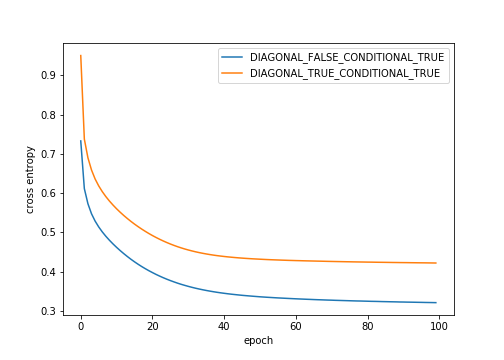
\includegraphics[width=.7\textwidth]{figures/trainning_history.png}
    \caption{Cross entropy loss for trainning networks. We trained networks to learn conditional probabilities \( P_c\{V | V^-\} \). The green line shows trainning dynamics using data generated with directions "left, right, up and down". The yellow line also takes diagonal directions into account, which has 8 directions in total. Naturally, since more directions implies higher complexity, the overall loss for yellow line is higher than green line.}
    \label{fig:trainning}
\end{figure}

The network consists of 31 convolutional layers. It has both down-sampling path for extracting high-level features and up-sampling path for recovering full resolution. The network is trained with mini-batches of size of 128, and  is optimized with Adam optimizer. The training runs for 100 epoches, with early stopping patience of 15 epoches. Figure \ref{fig:trainning} shows the cross entropy loss during training.

\section{Human Trajectory Simulation} \label{section:hms}

To acquire enough amount of data for trainning our netwrok is expensive, especially when we have to consider all possible motion changes for every cell in a grid map. For non-diagonal directions, there are \( 4\times4=16\) possible motion changes. For diagonal directions, it goes up to \( 8\times8=64\). To get statistically sound motion pattern probabilities, it requires to record human trajectories on many different maps over a long period of time. However, due to practical reasons, we are not able to get that much real data. Instead, we simulate human trajectories with A-star algorithm from 6 real world maps with a total free space area of ca. \( 6.6\times10^3 \, m^2 \). For each cell on the map, we try to sample 5 trajectories starting from that cell. With those trajectories, we can caculate motion pattern probabilities. Then we take random crops of size \( 32 \times 32 \) cells from the real world maps as network inputs, and their corresponding probabilities as outputs. 

% \figtwo{trajs\_through\_cell, trajs\_through\_cell, caption, trajs, htbp }

\begin{figure}[t]
\begin{tabular}{ll}
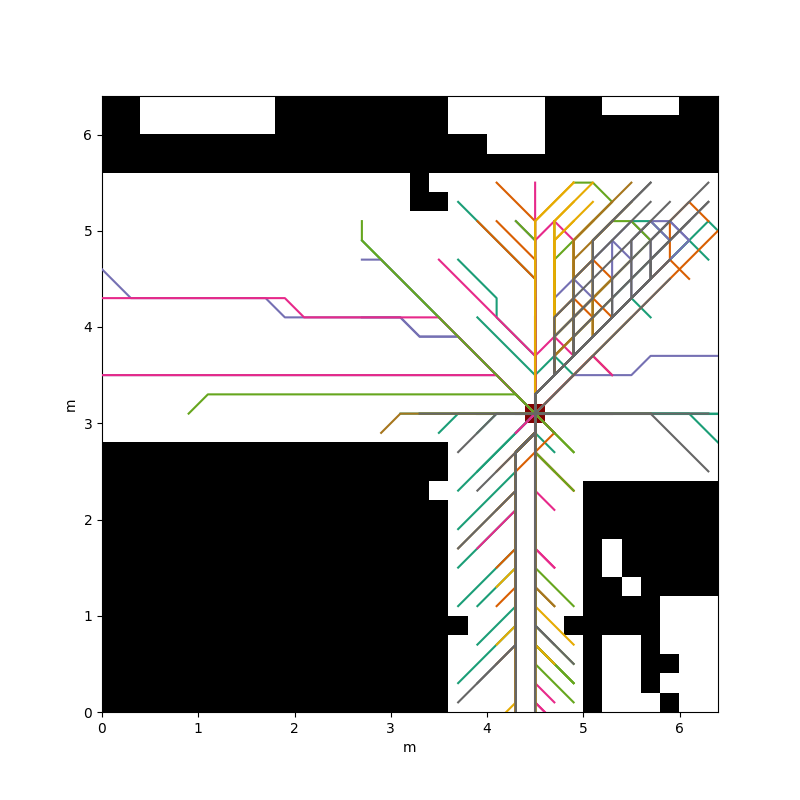
\includegraphics[width=0.48\textwidth]{figures/trajs_through_cell.png}
&
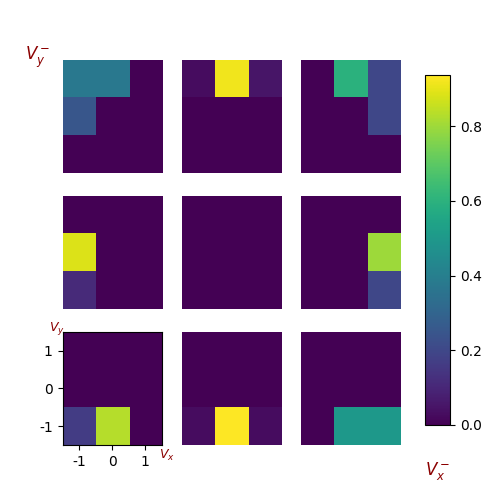
\includegraphics[width=0.48\textwidth]{figures/probs_on_that_cell.png}
\end{tabular}
\caption{\textbf{Left}: One example map crop as netwrok input. The map has size of \( 32 \times 32 \) cells, with resolution of \( 0.2m/cell\). It also shows trajectories that goes through the red cell. \textbf{Right}: Visualization of conditional probability \( P\{V | V^-\} \) for the red cell on left map. The axis shows velocities on \( x, y\) directions. Outter axes represent last velocity \( V^- \), and inner represent next velocity \( V \). One can see that \( P\{V=(-1, -1) | V^-=(-1, -1)\} = 0.21 \) and \( P\{V=(0, -1) | V^-=(-1, -1)\} = 0.79 \). This indicates that if a person reaches the red cell from upper right, it is very likely he will go downwards. }. 
\label{fig:trajs}
\end{figure}

Figure \ref{fig:trajs} shows one example of network input and the ground truth for one cell on the map. The number of samples we generated are summarized as follows:

\begin{center}
  \begin{tabular}{c|ccc}
    \hline
     & trainning & validation & test \\ \hline
    number of samples & 27,119 & 4,785 & 3,760\\
    \hline
  \end{tabular}
\end{center}

\section{Object Tracking using Bayesian Occupancy Filter}

Generally, Bayesian filter works in a recursive way and the filtering process can be decomposed into two stages: \textbf{prediction} and \textbf{correction}. For each time step, it firstly predicts the next state. After prediciton, when the new measurement is obtained, it corrects its prediction based on measurement. For Bayesian occupancy filter used in tracking applications, the state of world is represented by, for each cell on the grid map, the probabilities of cell's velocities and occupancy. However, the measurement gives information about only whether a cell is occupied or not at each time step. In order to make predicitions for the next time step, the filter has to infer velocities of each cell based on past occupancy information from measurements. Figure \ref{fig:correction} shows how BOFMP filter updates at one time step.


\begin{figure}[ht]
  \centering
    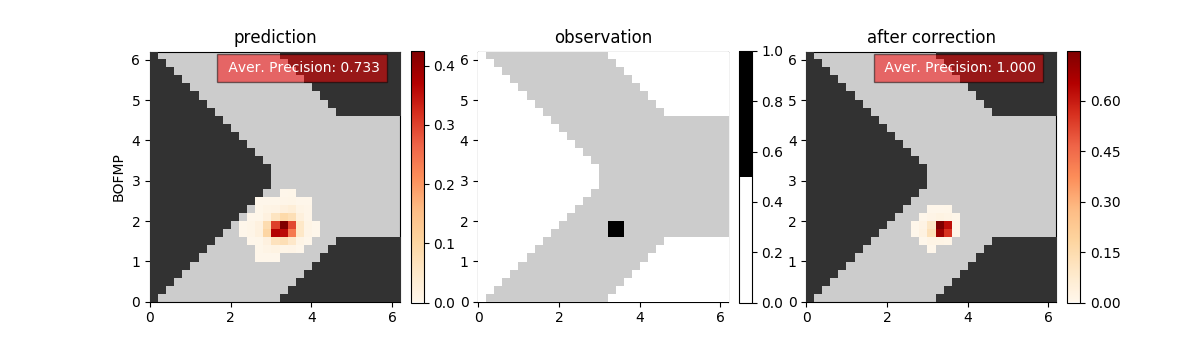
\includegraphics[width=\textwidth]{figures/correction_step.png}
    \caption{One filtering step of BOFMP filter. At last time step, the tracking object goes from up to down. Based on motion pattern, BOFMP predicts that there are possibilities that this object will trun to left-down and keep going downwards. After measurement shows that this obejct still goes downwards, BOFMP corrects its predictions and attenuates probabilities of turning left-down. Since the measurement adds additional information for BOFMP to make better predictions, the average precision increases after correction step.}
    \label{fig:correction}
\end{figure}

\section{Comparision between BOFUM and BOFMP}

To compare the performance of BOFUM and BOFMP, we consider two scenarios:

\begin{my_enumerate}
\item \textbf{tracking}. Measurements are given at each time step, and we evaluate consistency between occupancy predicton and the ground truth at every time step before a certain time point \( t \) .
\item \textbf{future prediction}. From time point \( t \) on, the measurement is no longer given. Then we evaluate occupancy predictions with ground truth for the next \( n \) time steps.
\end{my_enumerate}

The parameters of a BOF filter are:
\begin{my_enumerate}
\item \textbf{extent \( e\)}. It determines the maximum velocity of a cell. For example, if extent is 7, the velocities are in range  \( [-3, 3] \) cells/time step on both \( x \) and \( y \) axis. Since our neural network only models velocities within \( [-1, 1]\), we need firstly extend it to higher velocities. The details on how we do this will be explained in the thesis. 
\item \textbf{noise variance \( \delta^2\)}. Both BOFUM and BOFMP assume the tracking object has a constant velocity, with a Gaussian distributed acceleration noise. This parameter determines how likely an object accelerates or decelerate.
\item \textbf{omega \( \Omega \)}. In the correction step of BOF filters, measurments from sensors are incorporated into filter's prediction. Since sensor could be noisy, this parameter determines how much do we trust our measurements. The sensor used for our tracking application is laser rangefinder, which is rather physically reliable and therefore has a low \( \Omega \) value.
\end{my_enumerate}

The possible metrics that could be used for measuring the consistency between occupancy predicition and ground truth are: \textit{cross entropy}, \textit{f1 score} and \textit{average precision}.  We choose average precision as our metric and the reasons will be detailed in the thesis. To prove that our method is able to make predictions according to human motion pattern, we tune the parameters based on filter's performance for future predictions. For both filters, we randomly sample 100 sets of parameters from parameter ranges listed in Table \ref{table:param_range}, evaluate on tracking cases with time steps of 16 and caculate average precision for every time step over all tracking cases. Note that value range of noise variance $\delta^2$ for real data is higher than for simulated data. This is because in real data, there are higher uncertainties with human motion and sensor failures. The measurement is lost at time step \( t=9\), and we select the best set of parameters based on the average of average precisions for the next \( 8 \) time steps. 

\begin{table}[H]
\centering
  \begin{tabular}{c|c|c}
    \hline
     &   value range for simulated data & value range for real data \\ \hline
    \( e \) & \( \{3, 5, 7\} \) &  \( \{3, 5, 7\} \)\\
    \(  \delta^2\) & \( [0.1, 0.6]\) & \( [0.2, 0.7]\) \\   
   \( \Omega \) & \( [0.01, 0.2] \) & \( [0.01, 0.2] \)\\
   \hline
 \end{tabular}
\caption{Parameter ranges for BOF filters.}
\label{table:param_range}
\end{table}

\subsection{On simulated data}

We generated 500 tracking cases as validation set for tuning filter parameters and 500 tracking cases for test set. Validation and test cases are generated from different maps, and on each map, there are either one or two walking humans. We firstly tuned the parameters on validation set for BOFUM and BOFMP individually. Then we apply both filters with their best parameters on test set. The best set of parameters and its corresponding average precision from \( t=9 \) to \( t=16 \) on test data are listed in Table \ref{table:best_param_simulated}. Figure \ref{fig:simulated_test_data} shows mean of average precision over 500 test cases for each time step.

\begin{table}[H]
\centering  
\begin{tabularx}{\textwidth}{c|c|c|c|c|c}
    \hline
    & $ e $ & $ \delta^2 $ & $ \Omega $ & average precision for $t=8:16 $ & mean\\ \hline
    BOFUM & 7 & 0.556 & 0.0164 &  0.767  0.599  0.500    0.416  0.349  0.279  0.232  0.192 & 0.417 \\
    BOFMP & 7 & 0.373 & 0.0353 & 0.785  0.637  0.552  0.479  0.416  0.358  0.311  0.252 & 0.474 \\
   \hline
  \end{tabularx}
\label{table:best_param_simulated}
\caption{Best parameters for BOFUM and BOFMP on simulated data.}
\end{table}


\begin{figure}[ht]
  \centering
    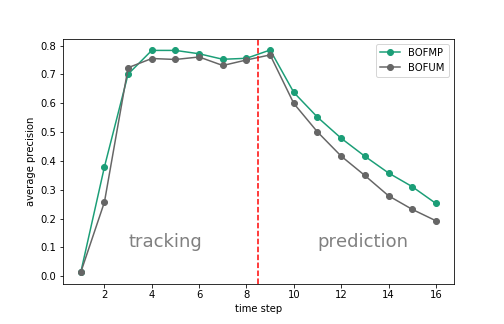
\includegraphics[width=.8\textwidth]{figures/test_on_simulated_data.png}
    \caption{Evaluation results on test data. The average precision for both filters start with values close to zero. Since we highly trust our measurments (low $\Omega$), both filters are able to successfully track the objects within 3 time steps. The fact that average precision keeps a high vaule from $t=3$ to $t=8$ indicates that both filters can predict very well for the next immediate time step. Starting from $t=9$ (see the red dash line), measurements are no longer given. The prediction is still accurate for the next time step ($t=9$), but decreases progressively over time.  This is expected, since without measurements, the state of world becomes more and more uncertain. Even though, we can see that our BOFMP have a higher average precision value than BOFUM at almost every time step, which indicates the improvements of our method in both tracking and future predicition stages.}
    \label{fig:simulated_test_data}
\end{figure}

Figure \ref{fig:tracking_simulated_data} shows how BOFUM and BOFMP perform tracking on one case from test data. In this example, a person is walking from the lower door towards upper door. The grey curve on the map shows the trajectory of the person. At $t=8$, the person walks with upwards velocity of 1 cell/time step. Both algorithms track the person very well with average precision of $1.0$. At $t=9$, the measurement is lost and future prediction stage of tracking starts. At $t=10$, BOFUM predicts that the person will still goes upwards, with a low possibility going other directions. However, since BOFMP knows there is a door above, it predicts that the person is also very likely going to that door, and therefore turns to upper left. At later time steps, BOFMP continues to predict occupancy probabilities towards upper door as well as other possible directions (i.e., door on the left and empty space on the right). On the contrary, BOFUM still propagates most occupancies upwards. At $t=16$, since the object accelerates to higher velocity, most of occupancy predictions of BOFMP are left behind the tracking object.
\begin{figure}[ht]
  \centering
    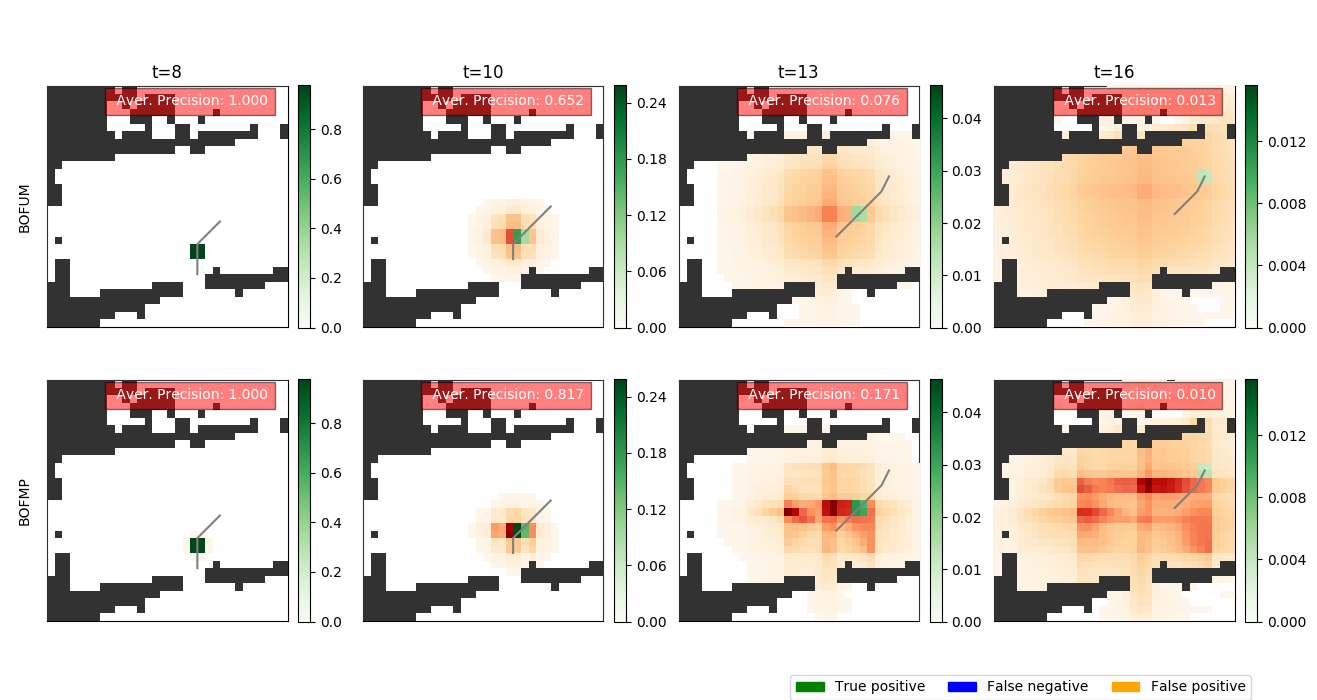
\includegraphics[width=\textwidth]{figures/tracking_sample_for_simulated_data.png}
    \caption{One example of tracking case from test data.}
    \label{fig:tracking_simulated_data}
\end{figure}

\subsection{On real data}

Although our neural network are trained on simulated human trajectories, we expect that our method also outperforms BOFUM on real tracking cases. We recorded human trajectories on two different ground plans by a laser rangefinder mounted on a robot. After processing raw laser data, we get 500 tracking cases for validation from one of the ground plans and 244 for test from the other. 



\textbf{Spatial blurring of motion probabilities}

The simulated trajectories do not always reflect real human's motion patterns. This is because, as shown in Figure \ref{fig:blur_idea}, humans are more flexible to decide when to make turns. 

\begin{figure}[ht]
  \centering
   \captionsetup{width=\linewidth}
    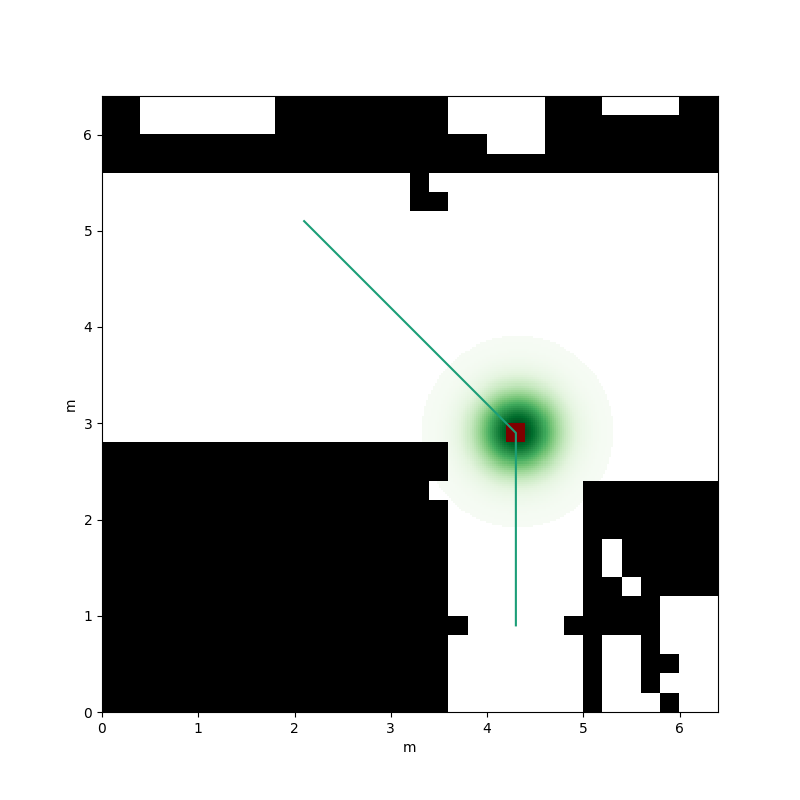
\includegraphics[width=.6\textwidth]{figures/blur_idea.png}
    \caption{A turn on simulated human trajectory. In order to reach the goal location in upper left corner, the simulated trajectory shows that a person will make a turn from going up to going up-left at location indicated by the red square. However, in real scenarios, a person is more flexible in deciding where to make that turn and he might turn at any location in the green area.}
    \label{fig:blur_idea}
\end{figure}

Therefore, to better adapt to real data, we introduce a techinique that blurs the motion probabilities  \( P_c\{V | V^-=v\} \) of a cell $c$ spatially into its neighbors if a \textit{turn} is detected. A \textit{turn} on cell $c$ for velocity $v^-$ is defined as:

\[ 
turn_c(v^-) = 
\begin{cases}
    True , & \text{if} \quad \argmax_v (P_c\{V=v | V^-=v^-\}) \, != \, v^- \\
    False,              & \text{otherwise}
\end{cases}
 \]


For each turn detected from motion pattern, we apply Gaussian blur spaitally to its neighbor cells' motion probability $P\{V | V^-=v^-\}$. As a consequence, another two parameters, blur extent \( blurExt \) and blur variance  \( blurVar \), are introduced and their value ranges are listed in Table \ref{table:spatial_blur_param_range}.


\begin{table}[H]
\centering  
\begin{tabularx}{.8\textwidth}{c|c|c}
    \hline
      &  \textit{value range } & \textit{note} \\ \hline
    \( blurExt \) & \( \{3, 5, 7, 9\} \) & \footnotesize{determines how far the Gaussian blur can reach} \\
     \( blurVar \) & \( [0.5, 2]\) & \footnotesize{ variance of the Gaussian kernel used for blurring} \\   
   \hline
  \end{tabularx}
\label{table:spatial_blur_param_range}
\caption{Parameters introduced by spatial blurring and their value ranges.}
\end{table}

\textbf{Motion keeping for future prediction}

Our proposed BOFMP, just like BOFUM, is \textit{memory-less}. That is to say, the last step of trakcing stage has absolute influence on future predictions, and the steps before the last step has no influence at all. In the real data we recorded, a time step equals to 0.25 second in real time. However, this short period of time is not able to summarize human's motion in the past time steps. Therefore, we propose to add moving average velocity of last few steps to the predicted velocity $P\{V_{pred}\}$, and then caculate next velocity $P\{ V \}$ from it. This process of incorporating moving average velocitiy is called as \textit{motion keeping}. It starts from the beginning of future prediction stage and the influence of moving average velocity is exponentially decreased over the following time steps.

Motion keeping also introduces new parameters. Assume the measurement is lost since time step $t_{lost}$, the new parameters are: 
\begin{my_enumerate}
\item \textbf{window size $w$}. It determines how many last time steps are considered when caculate moving average velocity .
\item \textbf{initial motion factor \( initMF\)}. This coefficent determines at the beginning of future predicition stage (i.e., $t=t_{lost}$), how much of moving average velocity $P\{V_{ma}\}$ is incorporated into predicted velocity $P\{V_{pred}\}$. 
\item \textbf{keep motion factor \( keepMF \)}. This constant is the base of the exponential function used to decrease moving average velocity $P\{V_{ma}\}$ over the following time steps. Therefore, for $t \geq t_{lost}$, 

\begin{align}
factor &= initMF \times keepMF^{(t-t_{lost})} \\
P\{V_{merge}\} &= factor \times P\{V_{ma}\} + (1-factor) \times P\{V_{pred}\}
\end{align}

\end{my_enumerate}

The value ranges of these parameters are listed in Table \ref{table:motion_keeping_param_range}. One example of tracking on real data using motion keeping is shown in Figure \ref{fig:keep_motion_idea}.
\begin{table}[H]
\centering  
\begin{tabularx}{.3\textwidth}{c|c}
    \hline
      &  \textit{value range } \\ \hline
    $w$ & \( \{2, 4, 6\} \)  \\
     $initMF$ & \( [0.3, 0.8]\) \\  
     $keepMF$ & \( [0.3, 0.8]\) \\    
   \hline
  \end{tabularx}
\label{table:motion_keeping_param_range}
\caption{Parameters introduced by motion keeping and their value ranges.}
\end{table}

\begin{figure}[ht]
\centering
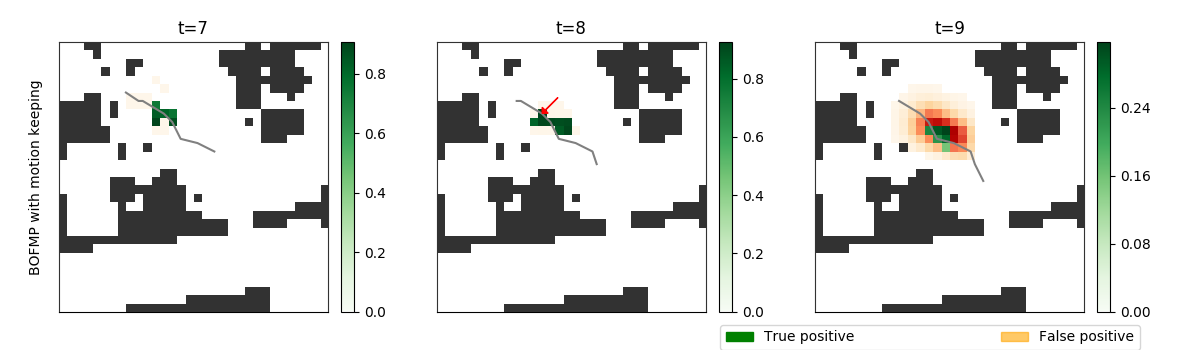
\includegraphics[width=\textwidth]{figures/moving_average_tracking.png}
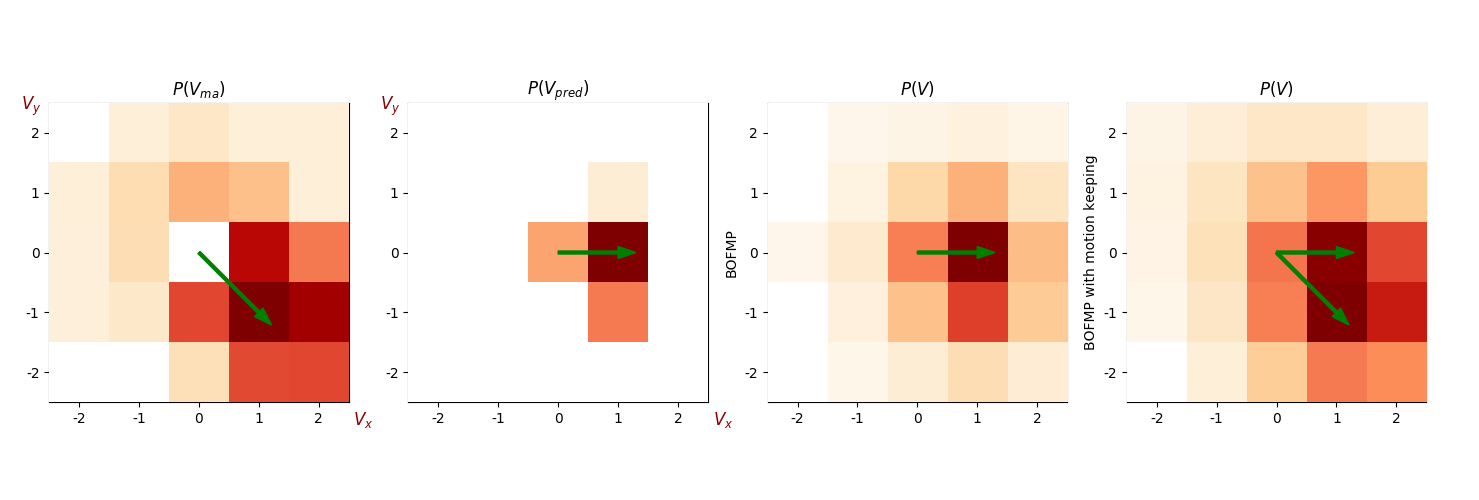
\includegraphics[width=\textwidth]{figures/moving_average_tracking_velocities_1.png}
\caption{\textbf{Up}: Three tracking steps of BOFMP with motion keeping. A person is walking from upper left towards lower right. The measurement is lost at $t=9$. \textbf{Down}: Velocities of the cell pointed by the red arrow at $t=8$. On each plot, the most possible direction is shown by the green arrows. Based on measurements from $t=7$ and $t=8$, the predicted velocity $P\{V_{pred}\}$ shows it is more likely the occupancy will propagates towards right for the next time step. However, past motion trend, which is represented by $P\{V_{ma}\}$, shows it is more likely to move to lower right. As a consequnce, BOFMP with motion keeping shows there are possibilities going both right and lower right, which is more realistic in this tracking example.}
\label{fig:keep_motion_idea}
\end{figure}


We randonly sample 100 sets of parameters for each scenario, evaluate them on validation set, and select the best set of parameters based on the mean of average precisions for the future prediction stage ($t=9:16$). The best parameters are shown in Table \ref{table:best_param_real}.

\begin{table}[H]
\footnotesize
\centering  
\begin{tabularx}{\textwidth}{c|c|c|c|c|c|c|c|c|c}
    \hline
    & $ e $ & $ \delta^2 $ & $ \Omega $ & \sml{blurExt} & \sml{blurVar} & $w$ & \sml{initMF} & \sml{keepMF}  & \footnotesize{mean a.p.}\\ \hline \hline
    BOFUM & 5 & 0.677 & 0.152  & - & - & - & - & - & 0.302   \\ \hline
    BOFMP & 5 & 0.649 & 0.191  & - & - & - & - & - & 0.321  \\
    \scriptsize{BOFMP spatial blurring} & 5 & 0.636 & 0.100  & 5 & 1.093 & - & - & - & 0.327  \\
    \scriptsize{BOFMP motion keeping} & 7 & 0.744 & 0.026  & - & - & 4 & 0.563 & 0.707 & 0.381  \\
   \hline
\end{tabularx}
\label{table:best_param_real}
\caption{Best parameters for BOFUM and BOFMP on real data.}
\end{table}

\normalsize
Then we apply each filter with its best parameters on test data of 244 tracking cases. Figure \ref{fig:real_test_data} shows the average precision for each time step, and Table \ref{table:real_test_data} lists the average precision in future prediction stage and their mean. Compared with BOFUM, our methods have performance gain of $29\%$, $31\%$ and $43\%$ respectively.

\begin{table}[H]
\footnotesize
\centering  
\begin{tabularx}{.8\textwidth}{c|c|c}
    \hline
    & average precision for $t=9:16$ & mean \\ \hline \hline
    BOFUM & 0.670   0.512  0.384  0.314  0.252  0.205  0.167  0.148  & 0.331   \\ \hline
    BOFMP & 0.705  0.570   0.468  0.424  0.351  0.336  0.305  0.255 & 0.427  \\
    \scriptsize{BOFMP spatial blurring} & 0.694  0.564  0.480   0.439  0.371  0.349  0.311  0.264 &  0.434  \\
    \scriptsize{BOFMP motion keeping} &  0.762  0.675  0.561  0.496  0.405  0.353  0.305  0.238 & 0.474  \\
   \hline
  \end{tabularx}
\label{table:real_test_data}
\caption{Future predictions for BOFUM and BOFMP on real data.}
\end{table}
\normalsize

\begin{figure}[ht]
  \centering
   \captionsetup{width=\linewidth}
    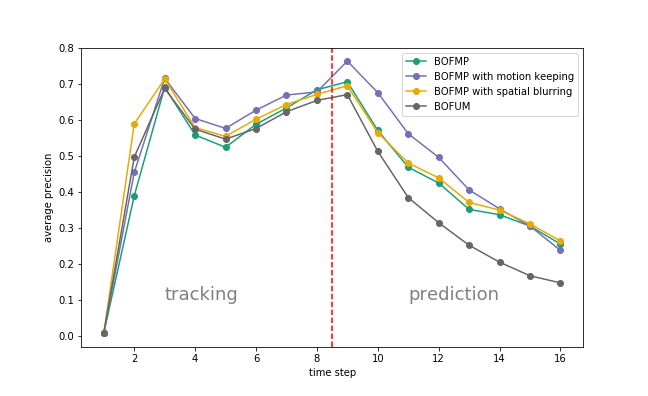
\includegraphics[width=.8\textwidth]{figures/test_on_real_data.png}
    \caption{Evaluation results on real test data. Like for simulated data, average precision starts with values close to zero, and increase rapidly over the next two time steps. From $t=3$ to $t=8$, average precisions keep rather stable at high values, which proves that filters predict very well for the next immediate step. In future prediction stage ($t=9:16$), average precisions decrease severely as time horizon increases, since the state of the world becomes more uncertain. However, our BOFMP and its variations are still better than BOFUM for every time step in this stage.}
    \label{fig:real_test_data}
\end{figure}

To conclude, we proposed a Bayesian occupancy filter that utilizes human motion pattern for tacking humans in indoor environments. The motion patterns are gained from a neural network which is trained on simulated human trajectories. Our proposed method outputforms BOFUM on both simulated and real tracking cases. One of the most important advantages of our method is that, although the motion pattern is derived from simulated data, it is applicable on real tracking scenarios.  











